\section{Theory}
\FloatBarrier % Now figures cannot float above section title

The method of calculating the plastic moment is introduced in the powerpoint of the Week 6 lecture. As shown in the figure below \autoref{f1}.

\begin{figure}
    \centering
    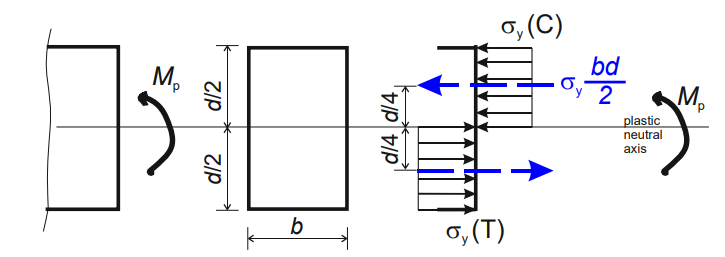
\includegraphics[]{./fig/11.png}
    \caption{plastic modules of rectangular section  }
    \label{f1}
\end{figure}

The plastic moment $M_p$ when all points in the section reached
yield stress $\sigma_y$ is caculated by:

\begin{equation} 
    M_p=\sigma_y\frac{bd}{2}(\frac{d}{4}+\frac{d}{4})
    \label{e1}
\end{equation}

Calculated from the data from \autoref{t1}, we get $M_p=8.67N \cdot m$.

There are three cases of collapse of plasticity of portal frame. We use virtual work method to caculate it.

\begin{figure}[htbp]
    \centering
    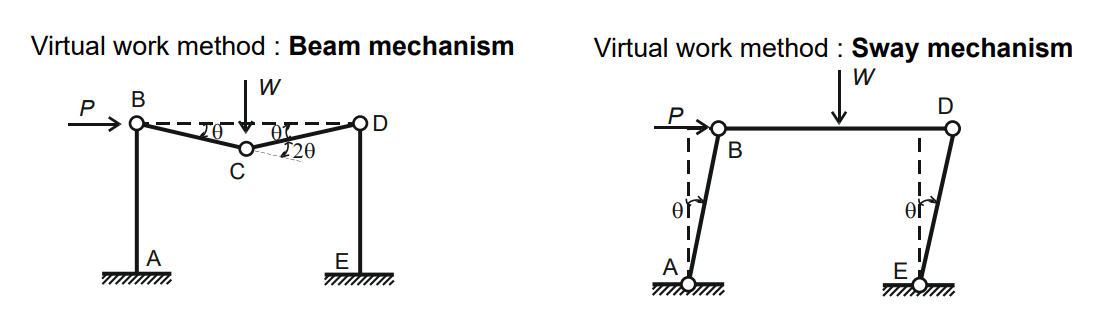
\includegraphics[width=10cm]{./fig/12.png}
    %\caption{plastic modules of rectangular section  }
    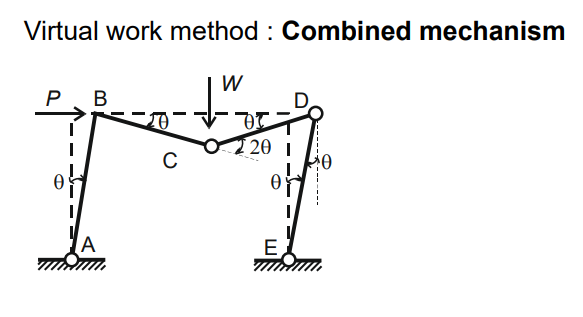
\includegraphics[width=5.5cm]{./fig/13.png}
    \caption{Three cases of collapse of plasticity of portal frame}
    \label{f2}
\end{figure}


$\bullet$ Beam mechanism: If $W>>P$, the hinges are likely to appear in B, C and D.



$\bullet$ Sway mechanism: If $P>>W$, the hinges are likely to appear in A, B, D and E.




$\bullet$ Combined mechanism: If P $\approx$ W, the smallest moment
is at B (as moments due to P
and W oppose each other), so
hinges form at other possible
locations. (The angle between ABC is $90^\circ$)

The virtual work method is: 

\begin{equation}
    \sum_i^{}{P_i\delta_i}=\sum_j^{}{M_j\theta_j}
    \label{e2}
\end{equation}

We noticed that the height (200mm) is equal to $\frac{2}{3}$ length (300mm). i.e. $H=\frac{2}{3}L$.

By using \autoref{e2}, we can get

$$
\left\{ \begin{array}{l}
	W\frac{\theta L}{2}=M_p\theta+M_p2\theta+M_p\theta \rightarrow W=\frac{8M_p}{L} (Beam)\\
	P\frac{2L}{3}\theta=M_p\theta+M_p\theta+M_p\theta+M_p\theta \rightarrow P=\frac{6M_p}{L} (Sway)\\
	P\frac{2L}{3}\theta+W\frac{\theta L}{2}=M_p\theta+M_p2\theta+M_p2\theta+M_p\theta \rightarrow 4P+3W=\frac{36M_p}{L} (Combined)\\
\end{array} \right. 
$$

Plot the relationships P-W on a graph

\begin{figure}[htbp]
    \centering
    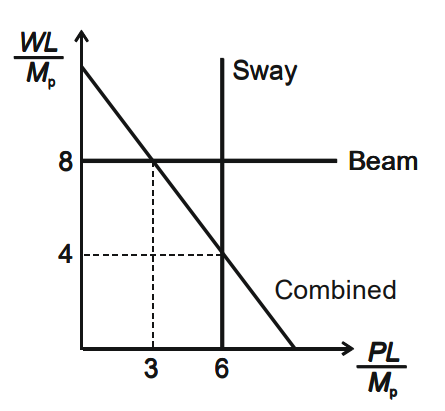
\includegraphics[width=6.5cm]{./fig/14.png}
    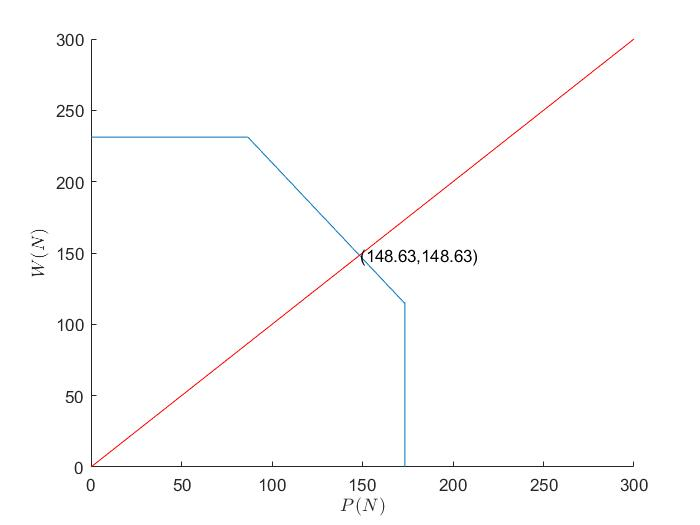
\includegraphics[width=8.5cm]{./fig/15.jpg}
    \caption{P-W graph}
    \label{f3}
\end{figure}



Substitude data from \autoref{t1} and \autoref{e1}, We have $\frac{M_p}{L}=28.9$ and the boundary of the graph is 

$$
\left\{ \begin{array}{l}
	W=\frac{8M_p}{L}=231.2\\
	P=\frac{6M_p}{L}=173.4\\
	4P+3W=\frac{36M_p}{L}=1040.4\\
\end{array} \right. 
$$

Plotting the three boundary lines with the applied load lines ($y=x$) on the graph, the following figure is obtained.

$$
\left\{ \begin{array}{l}
	4P+3W=1040.4\\
	P=W\\
\end{array} \right. 
$$
The solution to the equation is ($P=W=148.63$)
where the coordinates of the load line and the boundary line are (148.63,148.63\label{ee}).







